\documentclass{standalone}

\usepackage{tikz}
\usetikzlibrary{shapes, positioning, arrows.meta, calc, backgrounds, fit}

% default horizontal/vertical distance
\def\hdist{1.5}
\def\vdist{1.5}

\newcommand{\state}[2]{% #1: state label; #2: position
  \node (#1) [circle, inner sep = 0pt, minimum size = 10mm, text width = 10mm, align = center, draw, #2, font = \Large] {$#1$};
}

\newcommand{\transition}[4][]{% #2: start state; #3: end state; #4: transition label; #1: transition label position (optional)
  \draw[>=Stealth, ->] (#2) to node [rectangle, draw, above = 2pt, sloped, #1] {#4} (#3);
}

\begin{document}
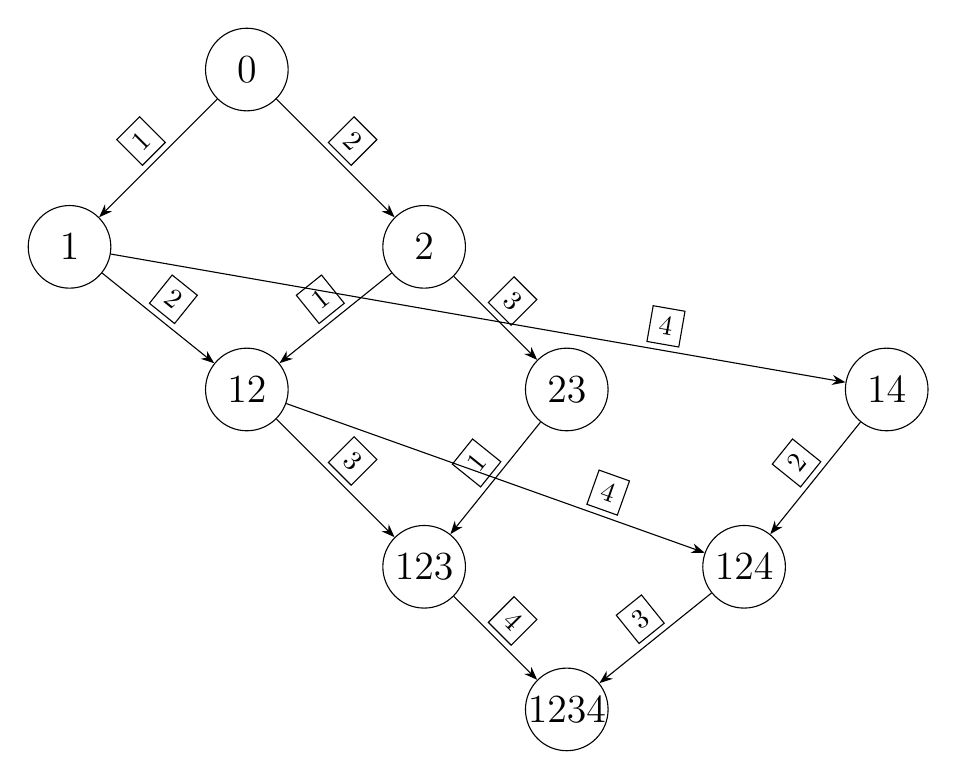
\begin{tikzpicture}[node distance = \vdist and \hdist]
  \state{0}{}
  \state{1}{below left = of 0}
  \state{2}{below right = of 0}

  \state{12}{below = 2*\vdist of 0}
  \state{23}{right = 2*\hdist of 12}
  \state{14}{right = 2*\hdist of 23}
  
  \state{123}{below = 2*\vdist of 2}
  \state{124}{right = 2*\vdist of 123}

  \state{1234}{below = 2*\vdist of 23}

  \transition{0}{1}{1}
  \transition{0}{2}{2}
  \transition{1}{12}{2}
  \transition{2}{12}{1}

  \transition{2}{23}{3}
  \transition{23}{123}{1}
  \transition{12}{123}{3}

  \transition[near end]{1}{14}{4}
  \transition[near end]{12}{124}{4}
  \transition{14}{124}{2}

  \transition{123}{1234}{4}
  \transition{124}{1234}{3}
\end{tikzpicture}
\end{document}
